\documentclass[11pt,a4paper]{article}

\usepackage[utf8x]{inputenc}   % omogoča uporabo slovenskih črk kodiranih v formatu UTF-8
\usepackage[slovene]{babel}    % naloži, med drugim, slovenske delilne vzorce

\usepackage[hyphens]{url}
\usepackage{hyperref}

\usepackage{graphicx}

\title{Optična razpoznava notnih znakov\\
\textsc{dispozicija diplomske naloge}}
\author{Matic Isovski\\
mi6568@student.uni-lj.si\\
\ \\
MENTOR: doc. dr. Luka Šajn \\
Fakulteta za računalništvo in informatiko\\ 
Univerza v Ljubljani
\date{\today}         
}



\begin{document}
\maketitle

\begin{abstract}
Dispozicijo diplomske naloge odprem z motivacijo, kakšno problematiko bom poskušal reševati, ter zakaj se mi tematika zdi zanimiva in pomembna. Sledi navajanje nekaj sorodnih del, jih na kratko opisal, ter utemeljitev povezave le teh z mojim diplomskim delom, ter zakaj se mi izbira mentorja zdi primerena. Predstavljen je tudi miselni diagram za izbrano temo, ter kaj bo diplomska naloga prispevala, kakšne rezultate pričakujem. Našteta so orodja ter metode, ki jih bom tekom diplome uporabljal. Proti koncu je predstavljena porazdelitev dela (aktivnosti, podaktivnosti ter njihova obdobja trajanja). Zaključim pa z preliminarnim kazalom diplomske naloge ter seznamom uporabljene literature.
\end{abstract}


\section{Motivacija za izbrano diplomsko temo}

Že od majhnih nog se ukvarjam z glasbo. Obiskoval sem glasbeno šolo, sodeloval pri raznih orkestrih, glasbenih skupinah, projektih itd. Sledilo je dolgo obdobje, ko se več nisem želel učiti igranja inštrumenta po notah in sem postal samouk. Sedaj mi je seveda žal, saj v branju not več nisem vešč in mi branje v realnem času lahko predstavlja problem. Aplikacija, ki bi omogočala razpoznavo not, bi mi zelo pomagala, tako pri delu, kakor pri učenju.

\subsection{Pregled področja in sorodnih del}

Nekaj sorodnih del:
\begin{itemize}
\item
Knjiga "Optical music sheet segmentation" \cite{omss}, v kateri je predstavljen je segmentacijski modul sistema O / sup 3 / MR (objektno orientirano optično prepoznavanje glasbe). Predlagani pristop temelji na sprejetju projekcij za ekstrakcijo osnovnih simbolov, ki predstavljajo grafični element glasbene notacije.
\item
Članek "The Challenge of Optical Music Recognition" \cite{tcomr}, opisuje izzive, ki jih predstavlja optično prepoznavanje glasbe. Najprej je opisan problem, nato pa je predstavljen splošen okvir za programsko opremo, ki poudarja ključne točke, ki jih je treba rešiti: identifikacija osebja, prepoznavanje glasbenih predmetov, klasifikacija glasbenih funkcij in glasbena semantika.
\item
Članek "New approaches to Optical Music Recognition" \cite{naomr}, opisujejo sistem se osredotoča na prepoznavo sestavljenih simbolov (akordi in skupine snopov).
\end{itemize}


\subsection{Zakaj je predlagani mentor primeren}

Za mentorja bi si lahko izbral doc. dr. Luko Šajna, saj ima veliko izkušenj na tem področju, izdal je tudi veliko člankov, ki bi mi tudi lahko bili zelo v pomoč, tako pri samem razumevanju področja, kot tudi pri implementaciji.


\section{Miselni diagram za izbrano temo diplomske naloge}

\begin{figure}[p]
\centerline{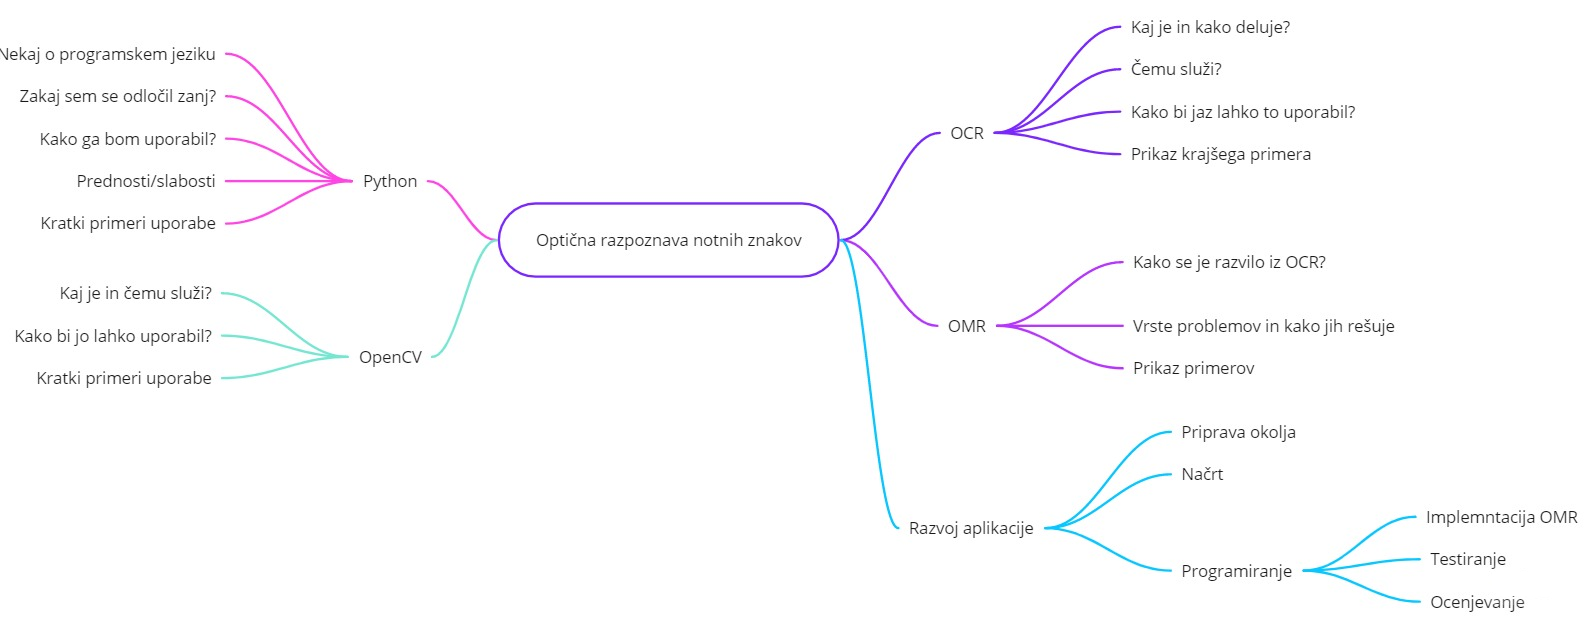
\includegraphics[scale=0.45, angle=90]{mindmap.png}}
\caption{Miselni vzorec za mojo diplomsko nalogo.}
\label{sl:mindmap}
\end{figure}

Na strani 3 lahko vidimo sliko, ki prikazuje miselni vzorec za mojo diplomsko nalogo (Slika \ref{sl:mindmap}), ki je razdeljen na pet delov: Pytgon (kjer bom pisal o tem programskem jeziku), OpenCV (kjer bom pisal o uporabi te knjižnjice), OMR (kjer bom predstavil tehnologijo optične prepoznave znakov), OCR (kjer bom predstavil podvejo), ter razvoj aplikacije (predstavil bom postopek izdelave aplikacije).



\section{Predvideni prispevki diplomske naloge}

Rezultat diplomske naloge bo podrobrobnejše razumevanje tehnologije optične prepoznave znakov, optične prepoznave glasbenih zapisov ter poznava primerov uporabe. Prav tako bo izdelana preprosta mobilna aplikacija, ki bo pomagala ljudem, ki jim branje not v realnem času predstavlja problem. Uporabnik bo slikal notni zapis in kot rezultat dobil njemu "uporabno" obliko zapisa (midi, tablature, ime tonov, itd.).


\section{Uporabljena metodologija}

Pri izdelavi sistema za prepoznavo notnih znakov bom uporabljal programski jezik Python, s knjižnico OpenCV si bom pomagal pri obdelovanju slik, konvolucijsko mrežo pa bom zgradil z uporabo knjižnice TensorFlow.


\section{Razdelitev potrebnega dela na aktivnosti}

\begin{enumerate}
\item Izbira tematike

Namen aktivnosti je dobro premisliti o zanimivih problematikah in izbrati temo, o kateri bi pisal v diplomski nalogi. Predvideno trajanje: 1 dan.
\item Izbira mentorja

Namen aktivnosti je pregled dela in publikacij profesorjev na FRI, ter izbrati mentorja, katerega usmeritev in delo je najbolj podobno izbrani tematiki. Predvideno trajanje: 1 dan.
\item Pisanje dispozicije

Namen aktivnosti je priprava dispozicie diplomskega dela. Predvideno trajanje: 4 dni.

\item Pisanje diplomske naloge
	\begin{enumerate}
	\item Teorija
	
	Namen podaktivnosti je pregled vseh virov, ki jih bom uporabil, ter iz njih črpati vsebino, ki je povezana z mojo tematiko. Predvideno trajanje: 2 meseca.
	\item Implementacija
	
	Namen podatkivnosti je razvijanje in testiranje aplikacije, ki uporablja OMR tehnologijo. Predvideno trajanje: 3 mesece.
	\end{enumerate}
	
\item Posvet z mentorjem

Namen aktivnosti je zadnji skupni pregled diplomskega dela z mentorjem ter pogovor o zagovoru. Predvideno trajanje: 1 teden.

\item Priprava na zagovor

Namen aktivnosti je priprava predstavitve ter časovna vaja. Predvideno trajanje: 1 dan.
\item Zagovor

Namen aktivnosti je zagovor diplomske naloge ter odgovarjanje na vprašanja. Predvideno trajanje: 15 minut.
\end{enumerate}

Nobenega dela nisem še zaključil, saj diplome ne bom pisal letos in je to zgolj načrt, ki ga bom lahko uporabu, če se bom res odločil za to tematiko. Predvideno skupno trajanje: 6 mesecev.

\section{Preliminarno kazalo}

\begin{enumerate}
\item Uvod

Kratko uvodna predstavitev diplomske naloge.
\item Python

Prestavitev in opis programskega jezika Python ter obrazložitev zakaj ga bom uporabljal.

\item OpenCV

Prestavitev in opis knjižnice OpenCv ter obrazložitev zakaj jo bom uporabljal.

\item OCR tehnologija
\begin{enumerate}
\item Predstavitev tehnologije

Podroben opis in razlaga ob primerih.

\item Kako se povezuje z OMR

Razlaga, kakšne so podobnosti, kako se je OMR razvilo iz OCR.
\end{enumerate}
\item OMR tehnologija

Podroben opis in razlaga ob primerih.

\item Razvoj sistema

Podrobno opis postopka izdelave aplikacije, v katero bom implementiral OMR.

\item Testirarnje

Opis prvih rezultatov, testiranja ter ocenjevanja. Predstavljeni bodo problemi, ter kako jih rešiti.

\item Zaključek

Opis končnih rezultatov, mojega zadovoljstva z rezultati ter zahvala mentorju ter vsem, ki so kakorkoli prispevali k diplomskemu delu.
\end{enumerate}


\bibliographystyle{plain}
\bibliography{literatura}

\end{document}  




